\section{HMT}
\subsection{General Introduction}
Segmentation of an image into unknown number of distinct and in some way homogeneous regions has been a fundamental issue in low level image analysis. There are many direct application of the algorithm, for example, segmentation of \gls{cti}, \gls{pet}, segmentation of \gls{nmr} images, and other applications in radar, satellite and agriculture. Many types of approaches has been in practice and in this paper a probabilistic method of segmentation is employed, \gls{hmm} based.

\subsection{Overview of Hidden Markov Model}
The \gls{hmt} was introduced by Crouse, Nowak and Baraniuk (1998). The context of their work was the modeling of statistical dependencies between wavelet coefficients in signal processing, for which variables are organized in a natural tree structure. Applications of such a model are: image segmentation, signal class cation, denoising and image document categorization \cite{durand2001statistical}.

A \gls{hmm} is a statistical Markov model in which the system being modeled is assumed to be a Markov process with unobserved (hidden) states. In a hidden Markov model, the state is not directly visible, but the output, dependent on the state, is visible. Each state has a probability distribution over the possible output tokens. Therefore, the sequence of tokens generated by an \gls{hmm} gives some information about the sequence of states. The adjective 'hidden' refers to the state sequence through which the model passes, not to the parameters of the model; the model is still referred to as a 'hidden' Markov model even if these parameters are known exactly \cite{jezicagent}. 
% from https://en.wikipedia.org/wiki/Hidden_Markov_model

The unifying ideas in using Markov Random Fields for vision are the following:
\begin{itemize}
	%\setlength\itemsep{1em}
	\item Images are dissected into an assembly of nodes that may correspond to pixels.
	\item Hidden variables associated with the nodes are introduced into a model designed to “explain” the values (colors) of all the pixels.
	\item  A joint probabilistic model is built over the pixel values and the hidden variables
	\item The direct statistical dependencies between hidden  variables are expressed by explicitly grouping hidden variables; these groups are often pairs depicted as edges in a graph.
\end{itemize}
These properties are illustrated in Figure \ref{fig:connectivity} below:
\begin{figure}[H]
	\centering
	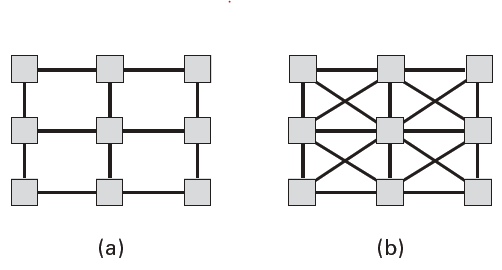
\includegraphics[width=0.7\textwidth]{fig/Connectivity.PNG}
	\caption{Graphs for Markov models in vision. (a) Simple 4-connected grid of image pixels. (b) Grids with greater connectivity
		here with the 8-connected pixel grid.}
	\label{fig:connectivity}
\end{figure}
%Figure \ref{fig:boat1} shows a boat.
The notation for image graphs is that the graph $G = (V, E)$ consists of vertices $V =(1, 2, . . . , i, . . . , N)$ corresponding, for example, to the pixels of the image, and a set of edges E where a typical edge is $(i, j)$, $i, j \in V$, and edges are considered to be undirected, so that $(i, j)$ and $(j, i)$ refer to the same edge. In the pixel graph of figure 1, the nodes are pixels, and a pair of pixels forms an edge in E if the two pixels share a common boundary.

The motivation for constructing such a graph is to connect the hidden variables associated with the nodes. For example, for the task of segmenting an image into foreground and background, each node i (pixel) has an associated random variable $X_i$ that may take the value 0 or 1, corresponding to foreground or background, respectively may take the value 0 or 1, corresponding to foreground or background, respectively. In order
to represent the tendency of matter to be coherent, neighboring sites are likely to have the
same label. So where $(i, j) \in E$, some kind of probabilistic bias needs to be associated with
the edge $(i,j)$ such that $X_i$ and $X_J$ tend to have the same label—both 0 or both 1. In fact, any
pixels that are nearby, not merely adjacent, are likely to have the same label. On the other
hand, explicitly linking all the pixels in a typical image, whose foreground/background
labels have correlations, would lead to a densely connected graph. That in turn would
result in computationally expensive algorithms. Markov models explicitly represent only
the associations between relatively few pairs of pixels—those pixels that are defined as
neighbors because of sharing an edge in E. The great attraction of Markov Models is that
they leverage a knock-on effect—that explicit short-range linkages give rise to implied
long-range correlations. Thus correlations over long ranges, on the order of the diameters of typical objects, can be obtained without undue computational cost.

Markov models are particularly useful as prior models for state variables Xi that are to
be inferred from a corresponding set of measurements or observations z = (z1, z2, . . . ,zi, . . . , zN). The observations z are themselves considered to be instantiations of a random variable Z representing the full space of observations that can arise.

123